\section{Modelo Numérico}
\label{sec:modelo-numerico}
O método proposto não introduz uma discretização nova às equações apresentadas na Seção \ref{sec:modelagem-matematica}. Ambos os domínios são resolvidos pelo núcleo implementado no MFSim. Assim sendo, a modelagem numérica é dividida em duas partes, tratando as particularidades de cada domínio, como acoplamento, interpolações e condições de contorno. O acoplamento pressão-velocidade também será detalhado, uma vez que sua ausência é objeto principal da formulação do filme. Esta seção descreve, primeiramente, os códigos comuns aos dois domínios, que são herdados do código, e posteriormente a descrição de cada um deles de forma separada.

\subsection{Visão Geral}
\label{sec:visao-geral-2}
O código adotado utiliza o Método de Volumes Finitos (\textit{FVM}) para a discretização de todas as equações de balanço \cite{versteeg2007}. As equações são integradas sobre cada volume de controle e os termos de divergência são convertidos em somatórios de fluxos através das faces, o que garante conservação discreta das grandezas transportadas no interior de cada nível de malha. A malha é cartesiana estruturada, com espaçamento uniforme dentro de um mesmo nível e razão de refino igual a dois entre níveis consecutivos.

Utiliza-se um arranjo de malha deslocada (\textit{staggered grid}), no qual as grandezas escalares, como pressão e fração volumétrica, são armazenadas no centro das células e grandezas vetoriais são armazenadas nas faces normais a cada componente. Esta configuração faz com que variações no gradiente de pressão sejam capturadas com mais facilidade, além de influenciar no estêncil utilizado nas interpolações entre níveis para cada variável \cite{versteeg2007,Villar2007}.

O termo advectivo e o difusivo são discretizados por meio de diferenças centradas de segunda ordem, sendo que o termo advectivo é resolvido na forma divergente e a difusão resolve o tensor completo. A escolha por diferenças de segunda ordem se dá pela natureza dos escoamentos utilizados no presente trabalho, sendo que os mesmos se desenvolvem principalmente por difusão. O avanço temporal utiliza um esquema chamado \textit{sbdf2}, com a advecção utilizando Adams-Bashforth de segunda ordem e a difusão totalmente implícita \cite{Martini2024}.

As condições de contorno são impostas por células fantasmas, por meio de camadas de células adjacentes a cada limite do domínio computacional, tais células são preenchidas de modo a representar a condição de Neumann ou Dirichlet desejadas na interface. Cada nível possui seu próprio conjunto de células fantasmas, de forma que no nível mais fino elas são preenchidas por meio de interpolações.

O acoplamento pressão velocidade utilizado é o método da projeção de Chorin \citep{Martini2024} ou método do passo fracionado. Tal método de acoplamento funciona de quatro etapas:

Primeiro resolve-se a equação de uma estimativa da velocidade, resolvendo Navier-Stokes com pressão vindo do tempo precedente:

\begin{align}
    \frac{3\vec{u}^{*} - 4\vec{u}^{n} + \vec{u}^{n-1}}{2\Delta t}
    + 2\,\nabla \cdot \left( \vec{u}\,\vec{u} \right)^{n}
    - \nabla \cdot \left( \vec{u}\,\vec{u} \right)^{n-1}
    \nonumber \\ = \frac{1}{\rho^{n+1}} \left[
        - \nabla p^{n}
        + \nabla \cdot \left( \mu^{n+1} \left( \nabla \vec{u}^{*} + (\nabla \vec{u}^{*})^{T} \right) \right) 
    \right]
    + \vec{f}_{\sigma}^{\,n+1}
    + \vec{f}_{ib}
    + \vec{g}
    \label{eq:predicao-velocidade}
\end{align}

As propriedades $\rho^{n+1}$ e $\mu^{n+1}$ são conhecidas nesta etapa.

O campo $\vec{u}^{*}$ não satisfaz a Eq. \ref{eq:continuidade-completa}. Impondo $\nabla \cdot \vec{u}^{\,n+1} = 0$ sobre a etapa de correção e subtraindo a Eq. \ref{eq:predicao-velocidade} da mesma equação escrita com $p^{n+1}$, obtém-se uma equação elíptica para a correção de pressão $p' = p^{n+1} - p^{n}$, Eq. \ref{eq:poisson}:

\begin{equation}
    \nabla \cdot \left( \frac{1}{\rho^{n+1}} \nabla p' \right)
    = \frac{3}{2\Delta t} \, \nabla \cdot \vec{u}^{*}
    \label{eq:poisson}
\end{equation}

Corrige-se então o campo de velocidade, Eq. \ref{eq:correcao-velocidade}:

\begin{equation}
    \vec{u}^{\,n+1} = \vec{u}^{*}
    - \frac{2\Delta t}{3} \, \frac{1}{\rho^{n+1}} \nabla p'
    \label{eq:correcao-velocidade}
\end{equation}

e, por fim, o campo de pressão, Eq. \ref{eq:correcao-pressao}:

\begin{equation}
    p^{n+1} = p^{n} + p'
    \label{eq:correcao-pressao}
\end{equation}

A Eq. \ref{eq:poisson} domina o custo do avanço, por exigir a solução de um sistema linear elíptico sobre todo o domínio, obtida no código por multigrid. É essa constatação que motiva a supressão da correção de pressão em $\Omega_f$, tratada na Seção \ref{sec:numerico-filme}.


A partir desses elementos nativos do código, tem-se particularidades de cada domínio, para a solução e acoplamento. 

\subsection{Escoamento Principal}
\label{sec:numerico-core}

O escoamento resolvido no \textit{coreflow} é monofásico, com $\rho$ e $\mu$ constantes e $\vec f_{\sigma}$ nulo, reduzindo a Eq. \ref{eq:predicao-velocidade}. O escoamento é representado pela Figura \ref{fig:escoamento_principal}. 

\begin{figure}[H]
    \centering
    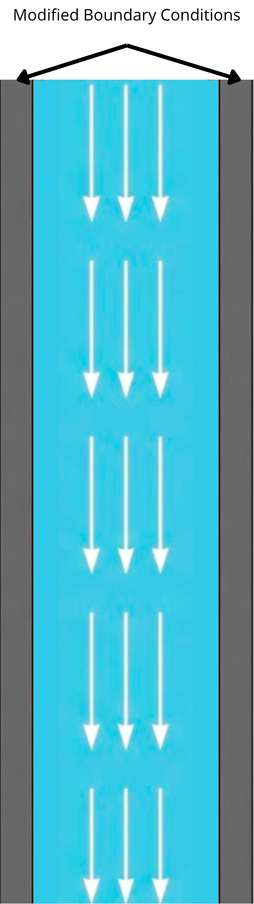
\includegraphics[width=0.2\textwidth]{imagens/principal_core.png}
    \caption{Escoamento principal com condições de contorno arbitrárias}
    \label{fig:escoamento_principal}
\end{figure}

O esquema continua utilizando a estrutura do multigrid para a solução da pressão, com o passo fracionado completo. O multigrid utiliza a estrutura dos níveis físicos e virtuais escolhidos para este escoamento.

A principal mudança neste domínio é o acoplamento, feito por meio das condições de contorno de parede. 

\subsubsection{Condições de Contorno}
\label{sec:condições_de_contorno}

A condição de contorno ideal para transmitir o efeito do filme para o escoamento principal foi um dos objetos de estudo deste trabalho. Sendo assim, várias condições foram testadas e seus resultados comparados, a Tabela \ref{tab:condicoes} mostra cada uma das condições e seus tipos:

\begin{table}[htbp]
  \centering
  \caption{Condições de contorno da simulação.}
  \label{tab:condicoes}
  \begin{tabular}{l l l}
    \toprule
    \textbf{Tipo de condição} & \textbf{Nome} & \textbf{Valor} \\
    \midrule
    Dirichlet   & Sem acoplamento & $v_{wall} = 0$ \\

    Dirichlet   & velocidade igual a interface     & $v_{wall} = v_{interface}$ \\

    Neumann     & igualdade das derivadas     & $\frac{\partial v}{\partial x}\|_{wall} = \frac{\partial v}{\partial x}\|_{interface}$ \\

    Neumann   & Adapted Navier-Slip     & $\frac{\partial v_{wall}}{\partial x} = \frac{v_{interface}}{\Lambda_{film}}$ \\

    Dirichlet   & Adapted Navier-Slip Dirichlet & $v_{wall} = \frac{\mu_{core} - \mu_{film}}{|\mu_{core} - \mu_{film}|} \cdot \Lambda_{film} \frac{\partial v_{film}}{\partial x}$ \\
    \bottomrule
  \end{tabular}
\end{table}

A primeira condição de contorno foi utilizada apenas para verificar como o gás se comporta sem a presença do fluido e quanto de erro isso gera, também verifica a diferença entre o acoplamento de uma via e os acoplamentos de duas vias.

A segunda condição iguala a velocidade da parede à velocidade da interface do escoamento, sendo essa a primeira tentativa realizada de acoplamento filme-core, se mostrando inviável, como é discutido posteriormente.

A terceira condição de contorno imposta visa reproduzir a tensão de cisalhamento na interface entre fluidos. Uma vez que o escoamento se desenvolve quase que puramente por difusão, já que não existe velocidade na direção normal ao mesmo nos escoamentos utilizados no presente trabalho, foram testadas três formas de se medir a derivada na interface, ilustradas na Figura \ref{fig:medicao_normal}.

\begin{figure}[H]
    \centering
    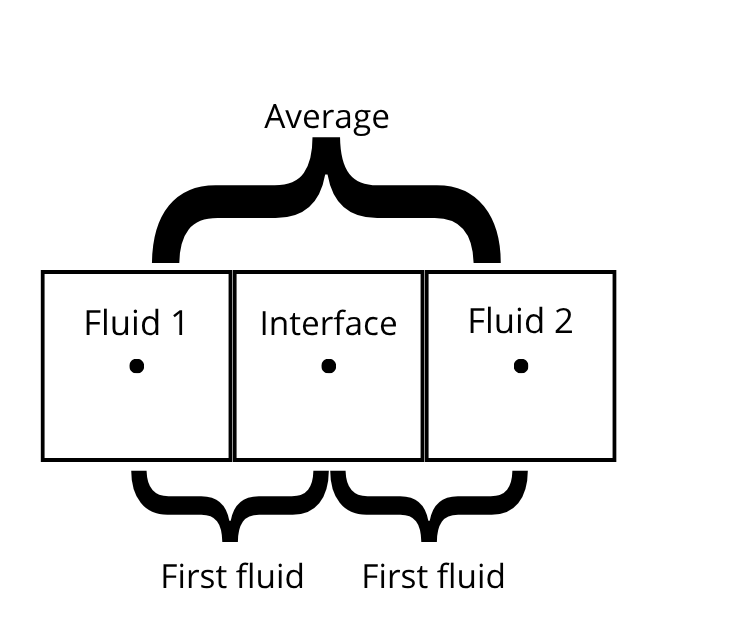
\includegraphics[width =0.6\textwidth]{imagens/medicao_normal.png}
    \caption{Ilustração dos três casos testados para obter a derivada na interface, sendo que as condições são upwind backwind e uma média centrada}
    \label{fig:medicao_normal}
\end{figure}


Sendo assim foram feitas três tentativas de se obter a tensão cisalhante na interface. A primeira foi utilizar a última célula de filme e a célula de interface, dando mais ênfase à influência do filme, em simetria, também considerou-se o oposto, uma célula de interface e uma célula de fluido principal. Considerou-se também uma diferença centrada, utilizando uma célula de filme e uma de fluido principal para estimar a derivada na interface.

A condição de Navier-Slip adaptada surgiu a partir da manipulação da condição original de deslizamento de Navier, dada pela Eq. \ref{eq:Navier-Slip}

\begin{equation}
    v_{wall} + b\frac{\partial v}{\partial x}\|_{wall} = 0
    \label{eq:Navier-Slip}
\end{equation}

Nessa equação b é chamado de comprimento de deslizamento, e representa o comprimento equivalente ao qual o fluido está deslocado. A Figura \ref{fig:Navier-slip} mostra o efeito de vários comprimentos de deslizamento. Um ramo da mecânica dos fluidos que estuda muito essas condições é o de nanofluidos \citep{Wang2021}, os nanofluidos apresentam deslizamento relativos às paredes de acordo com várias características do fluido e da parede, uma delas é a afinidade química do material da parede com o fluido. Um exemplo disso é quando um nanofluido a base d'água é transportado ao longo de uma parede hidrofílica, o fluido se desenvolve mais do que ele se desenvolveria na presença de uma parede normal, sendo assim o comprimento de deslizamento deve refletir esse deslocamento. Por outro lado, se este mesmo fluido está em contato com uma superfície hidrofóbica, ele se desenvolverá menos que caso estivesse em contato com uma parede normal, levando a um comprimento de deslizamento negativo. 

\begin{figure}[H]
    \centering
    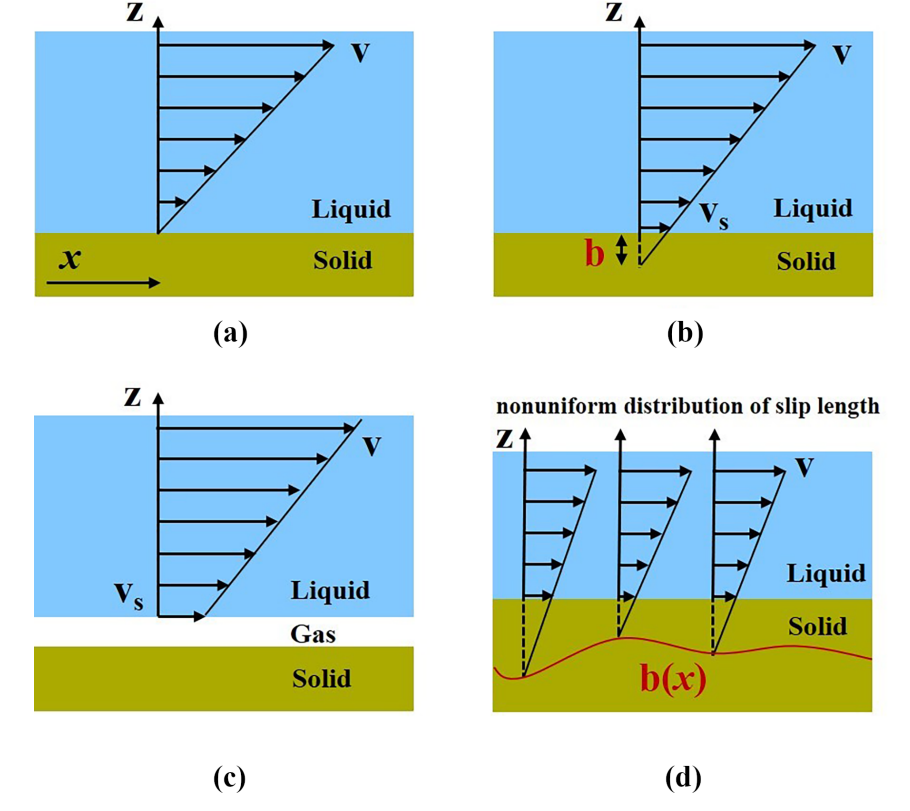
\includegraphics[width=0.7\textwidth]{imagens/navier-slip.png}
    \caption{Representação do modelo de deslizamento de Navier (Navier-Slip) apresentando o que o comprimento de deslizamento representa. Figura de \citet{Wang2021}}
    \label{fig:Navier-slip}
\end{figure}

A analogia feita no parágrafo anterior pode ser estendida a filmes finos: um filme com viscosidade maior que o fluido principal faz com que o escoamento obtenha uma velocidade terminal menor que caso o fluido principal estivesse sozinho na tubulação. Na condição oposta, usada nos casos de filme de lubrificação - em transporte de petróleo por exemplo -, o filme com menor viscosidade que o principal faz com que ele desenvolva uma velocidade terminal maior no escoamento. Este último caso faz com que seja possível observar um deslizamento do escoamento principal em relação às paredes, o mesmo efeito que se observa ao movimentar-se sobre superfícies lubrificadas.

Utilizando os resultados obtidos e a analogia apresentada, desenvolveu-se a condição de Navier-Slip com Dirichlet. Essa condição visa sanar uma limitação do método de fronteira imersa implementado no software utilizado, o código só consegue aplicar condições de primeira espécie.

Os resultados de cada condição de contorno são analisados separadamente nos resultados, para cada um dos escoamentos.


\subsection{Escoamento do Filme}
\label{sec:numerico-filme}
O domínio do filme é significativamente menor que o do escoamento principal. O tamanho exato do mesmo deve ser mensurado, tanto com análises de independência de malha quanto mensurando a altura esperada de ondas no filme, de forma que todo o conteúdo do fluido 1 deve permanecer confinado no domínio sem remalhagem.

O domínio do filme é representado pela Figura \ref{fig:dominio_filme}, as condições nas faces que encontram as paredes do domínio computacional ou a fronteira imersa são de não deslizamento, com velocidade zero para essas paredes. As condições de contorno para as faces internas ao domínio são fornecidas pelos níveis intermediários para a velocidade, utilizando a interpolação para as ghost cells apresentada por \citet{Villar2007}. Essas interpolações garantem o acoplamento do core flow para o filme. 

\begin{figure}[H]
    \centering
    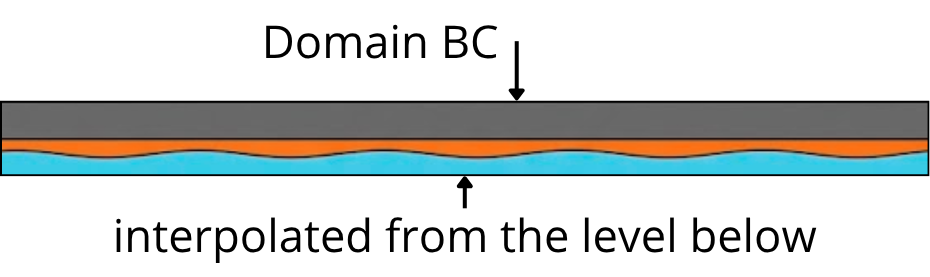
\includegraphics[width=0.5\textwidth]{imagens/filme-domain.png}
    \caption{Domínio do filme com as condições de contorno aplicadas}
    \label{fig:dominio_filme}
\end{figure}


O acoplamento pressão velocidade não é resolvido no domínio do filme, uma vez que a pressão é inteiramente fornecida pelo escoamento principal, assim sendo o acoplamento mostrado se resume à primeira equação, que ao em vez de fornecer uma estimativa para a velocidade, fornece seu valor para o próximo passo de tempo.

No domínio do filme o tratamento escolhido para o problema bifásico foi o \textit{VOF}.
A massa específica e viscosidade são funções do campo de volume fracionário $f$, que representa a fração de volume do fluido 1 em cada célula do domínio computacional. As equações de transporte do volume fracionário são resolvidas utilizando o método VOF, com reconstrução geométrica da interface, a equação de transporte de $f$ é representada pela Eq. \ref{eq:transporte-f}.

\begin{equation}
    \frac{\partial f}{\partial t} V + F_{net} = \int_{V} c \vec{\nabla} \cdot \vec{u} dv,
    \label{eq:transporte-f}
\end{equation}

sendo $F_{net}$ o fluxo líquido de fração volumétrica através das faces.
A Eq. \ref{eq:transporte-f} é resolvida pelo esquema conservativo com separação direcional proposto por \citet{Weymouth2010}. A cada passo de tempo são executadas três varreduras unidimensionais, uma por direção $d$, com permutação cíclica da ordem entre passos consecutivos para evitar viés direcional. O termo $c$ é aproximado por \citet{Weymouth2010} como função indicadora $c^*$ na célula:

\begin{equation}
    c^* =
    \begin{cases}
        1, & f > 1/2 \\
        0, & \text{caso contrário,}
    \end{cases}
    \label{eq:indicadora-wy}
\end{equation}


Após a obtenção de $f$ no domínio, os campos de $\rho$ e $\mu$ são reconstruídos utilizando Eq. \ref{eq:rho-reconstruido} e Eq. \ref{eq:mu-reconstruido}:

\begin{equation}
    \rho = \rho_1^f \cdot \rho_2^{1-f}
    \label{eq:rho-reconstruido}
\end{equation}

\begin{equation}
    \mu = f \mu_1 + (1-f) \mu_2
    \label{eq:mu-reconstruido}
\end{equation}

Sendo $\mu$ reconstruído com a formulação clássica e $\rho$ reconstruído com média geométrica que suaviza o gradiente na interface, de forma a evitar saltos abruptos e problemas de convergência. 

A tensão superficial é tratada como força de campo pelo modelo \textit{Continuum Surface Force} \citep{Brackbill1992}, Eq.\ref{eq:csf}: 

\begin{equation}
    \vec{f}_{\sigma} = \frac{\sigma \kappa \nabla f}{\langle \rho \rangle},
    \label{eq:csf}
\end{equation}

na qual $\sigma$ é a tensão superficial, $\kappa$ é a curvatura obtido a partir do método mostrado por \citet{Shirani2004} e ${\langle \rho \rangle = \frac{\rho_1 + \rho_2}{2}}$ que é a ponderação por massa específica que faz com que a aceleração resultante deste termo dependa da média das fases, sem saltos.


\subsection{Avanço temporal}
\label{sec:passo-tempo}
Para garantir a estabilidade dos métodos numéricos na solução de sistemas lineares, existem na literatura diversas análises que verificam os critérios de estabilidade desses sistemas baseados nos métodos que os resolvem. Tais critérios geralmente nascem de análises gerais como o método de análise de estabilidade de Von Neumann ou junto com os métodos numéricos específicos, como o encontrado em \citet{Brackbill1992}. Os critérios de passo de tempo utilizados neste trabalho são mostrados na Eq. \ref{eq:criterio_de_Brackbill} e Eq \ref{eq:criterio_advectivo}.

\begin{equation}
    \Delta t_{capilar} \leq \sqrt{\frac{\rho_{eq}\,\Delta x^3}{2 \pi \sigma}}
    \label{eq:criterio_de_Brackbill}
\end{equation}

\begin{equation}
    \Delta t_{advectivo} = CFL \cdot \frac{1}{\dfrac{u_{max}}{\Delta x} + \dfrac{v_{max}}{\Delta y} + \dfrac{w_{max}}{\Delta z}}
    \label{eq:criterio_advectivo}
\end{equation}

Sendo $\rho_{eq}$ a mesma ponderação de massa utilizada por \citet{Brackbill1992}, ou seja $\rho_{eq} = \langle\rho\rangle$.

O critério difusivo não é utilizado. Isso se dá em razão do método de discretização temporal que toma este termo como totalmente implícito.

O escoamento principal utiliza apenas a Eq. \ref{eq:criterio_advectivo}, por não ter tensão superficial, enquanto o filme utiliza ambas de forma que o passo de tempo final para este domínio é mostrado na Eq. \ref{eq:passo_final}.

\begin{equation}
    \Delta t_{film} = \min(\Delta t_{capilar}, \Delta t_{advectivo})
    \label{eq:passo_final}
\end{equation}

Por terem critérios e refino de malha diferentes, os domínios terão necessariamente passos de tempo diferentes. A sincronização entre esses passos de tempo é feita por meio do seguinte algoritmo:

\begin{equation}
    \begin{aligned}
        N_{passos} &= \left\lceil \frac{\Delta t_{core}}{\Delta t_{film}} \right\rceil \\
        \delta t_{film} &= \frac{\Delta t_{core}}{N_{passos}}
    \end{aligned}
    \label{eq:sincronizacao_dt}
\end{equation}

Sendo $\lceil \cdot \rceil$ a função teto, que arredonda o quociente para o menor inteiro maior ou igual a ele, de forma que o passo de tempo efetivo do filme, $\delta t_{film}$, seja sempre menor ou igual ao passo de tempo calculado, $\Delta t_{film}$, garantindo que os critérios de estabilidade sejam atendidos.

Dessa forma, o domínio do filme avança $N_{passos}$ passos de tempo valendo $\delta t_{film}$ em cada loop do código, sendo que ao final de cada passo de tempo global, tanto o filme quanto o \textit{coreflow} estão no mesmo tempo físico.

